%%%%%%%%%%%%%%%%%%%%%%%%%%%%%%%%%%%%%%%%%%%%%%%%%%%%%%%%%%%%%%%%%%%%%%%%%%%%%%%
% Memorial para concurso público de Professor Doutor na USP.
%
% Formatação inspirada em:
% * https://tug.org/pracjourn/2008-1/mori/mori.pdf
% * https://github.com/santisoler/phd-thesis
% * https://github.com/compgeolab/dissertation-template
%%%%%%%%%%%%%%%%%%%%%%%%%%%%%%%%%%%%%%%%%%%%%%%%%%%%%%%%%%%%%%%%%%%%%%%%%%%%%%%

%%%%%%%%%%%%%%%%%%%%%%%%%%%%%%%%%%%%%%%%%%%%%%%%%%%%%%%%%%%%%%%%%%%%%%%%%%%%%%%
% Set a class and import packages
\documentclass[10pt,a4paper,oneside]{book}

% Variables
\newcommand{\Year}{2022}
\newcommand{\Title}{Memorial para concurso público - Professor Doutor em Geofísica - IAG/USP}
\newcommand{\Author}{Leonardo Uieda}
\newcommand{\Email}{Leonardo.Uieda@liverpool.ac.uk}
\newcommand{\ORCID}{0000-0001-6123-9515}
\newcommand{\ResearcherID}{G-3258-2012}
\newcommand{\GoogleScholar}{qfmPrUEAAAAJ}
\newcommand{\Lattes}{8939551682050504}

% Variables for easier typing of some names
\newcommand{\UHM}{University of Hawai`i at M\={a}noa}
\newcommand{\UERJ}{Universidade do Estado do Rio de Janeiro}

% Names for citing coauthors
\newcommand{\Me}{\textbf{Uieda, L}}
\newcommand{\Val}{Barbosa, VCF}
\newcommand{\Bi}{Oliveira Jr, VC}
\newcommand{\Paul}{Wessel, P}
\newcommand{\Joaquim}{Luis, J}
\newcommand{\Remko}{Scharroo, R}
\newcommand{\Florian}{Wobbe, F}
\newcommand{\Walter}{Smith, WHF}
\newcommand{\Dongdong}{Tian, D}
\newcommand{\Bridget}{Smith-Konter, B}
\newcommand{\Eric}{Xu, X}
\newcommand{\David}{Sandwell, DT}
\newcommand{\Carla}{Braitenberg, C}
\newcommand{\Naomi}{Ussami, N}
\newcommand{\Manoel}{D'Agrella-Filho, MS}
\newcommand{\JB}{Silva, JBC}
\newcommand{\Dai}{Sales, DP}
\newcommand{\Figura}{Melo, FF}
\newcommand{\Dio}{Carlos, DU}
\newcommand{\BragaVale}{Braga, MA}
\newcommand{\YLi}{Li, Y}
\newcommand{\Angeli}{Angeli, G}
\newcommand{\Peres}{Peres, G}
\newcommand{\Everton}{Bomfim, EP}
\newcommand{\Eder}{Molina, E}
\newcommand{\Gomes}{Gomes, AAS}
\newcommand{\Santiago}{Soler, SR}
\newcommand{\Agustina}{Pesce, A}
\newcommand{\Gimenez}{Gimenez, ME}
\newcommand{\Kristoffer}{Hallam, KAT}
\newcommand{\Guangdong}{Zhao, G}
\newcommand{\Bo}{Chen, B}
\newcommand{\JLiu}{Liu, J}
\newcommand{\LChen}{Chen, L}
\newcommand{\RGuo}{Guo, R}
\newcommand{\MKaban}{Kaban, MK}
\newcommand{\Lindsey}{Heagy, LJ}
\newcommand{\Lion}{Krischer, L}
\newcommand{\Rene}{Gassmoeller, R}
\newcommand{\Bane}{Sullivan, CB}
\newcommand{\Jens}{Klump, JF}
\newcommand{\LBarba}{Barba, LA}
\newcommand{\JBazan}{Bazan, J}
\newcommand{\JBrown}{Brown, J}
\newcommand{\RGuimera}{Guimera, RV}
\newcommand{\MGymrek}{Gymrek, M}
\newcommand{\AHanna}{Alex Hanna}
\newcommand{\KHuff}{Huff, KD}
\newcommand{\DKatz}{Katz, DS}
\newcommand{\CMadan}{Madan, CR}
\newcommand{\KMoerman}{Moerman, KM}
\newcommand{\KNiemeyer}{Niemeyer, KE}
\newcommand{\JPoulson}{Poulson, JL}
\newcommand{\PPrins}{Prins, P}
\newcommand{\KRam}{Ram, K}
\newcommand{\ARokem}{Rokem, A}
\newcommand{\Arfon}{Smith, AM}
\newcommand{\GThiruvathukal}{Thiruvathukal, GK}
\newcommand{\KThyng}{Thyng, KM}
\newcommand{\BWilson}{Wilson, BE}
\newcommand{\Yehudi}{Yehudi, Y}
\newcommand{\Remi}{Rampin, R}
\newcommand{\Hugo}{van Kemenade, H}
\newcommand{\MattTurk}{Turk, M}
\newcommand{\Shapero}{Shapero, D}
\newcommand{\Anderson}{Banihirwe, A}
\newcommand{\Leeman}{Leeman, J}
\newcommand{\JEbbing}{Ebbing, J}
\newcommand{\AGuy}{Guy, A}
\newcommand{\JFarquharson}{Farquharson, J}
\newcommand{\AKushnir}{Kushnir, A}
\newcommand{\FWadsworth}{Wadsworth, F}
\newcommand{\LPerozzi}{Perozzi, L}
\newcommand{\MWieczorek}{Wieczorek, MA}
\newcommand{\LLi}{Li, L}
\newcommand{\Ricardo}{Trindade, RIF}

\usepackage[utf8]{inputenc}
\usepackage[T1]{fontenc}
\usepackage[brazil]{babel}
\usepackage[width=150mm,top=30mm,bottom=30mm,headsep=10mm,headheight=5mm]{geometry}
\usepackage{graphicx}
\usepackage{amssymb}
\usepackage{amsmath}
\usepackage{hyperref}
% create fancy headers
\usepackage{fancyhdr}
% commands for managing dates and its formats
\usepackage{datetime2}
% improved urls with proper hyphenation
\usepackage{xurl}
% Import enumitem to customize descriptions in license.tex
\usepackage{enumitem}
% Tweak the look of captions
\usepackage{caption}
% To control the style of section titles
\usepackage{titlesec}
% Add the bibliography to the table of contents
\usepackage[nottoc,chapter]{tocbibind}
\usepackage[round,authoryear,sort]{natbib}
% show dois as links on references
\usepackage{doi}
% Icon fonts (requires using xelatex or luatex)
\usepackage{fontawesome5}
\usepackage{academicons}
\usepackage{fontspec}
% Set fonts (requires compilation with xelatex)
\usepackage{fontspec}
\usepackage{microtype}
% To make fancy text boxes
\usepackage{xcolor}
\usepackage[framemethod=tikz]{mdframed}
% For fancy and multipage tables
\usepackage{tabularx}
\usepackage{ltablex}
% To define custom environments
\usepackage{environ}
\usepackage{setspace}
%%%%%%%%%%%%%%%%%%%%%%%%%%%%%%%%%%%%%%%%%%%%%%%%%%%%%%%%%%%%%%%%%%%%%%%%%%%%%%%

%%%%%%%%%%%%%%%%%%%%%%%%%%%%%%%%%%%%%%%%%%%%%%%%%%%%%%%%%%%%%%%%%%%%%%%%%%%%%%%
% Configuration of the document

\setmainfont[%
  Path = fonts/notoserif/,
  UprightFont = NotoSerif-Regular,
  BoldFont = NotoSerif-Bold,
  ItalicFont = NotoSerif-Italic,
  Extension = .ttf
]{NotoSerif}

% Increase the line spacing
\SetSinglespace{1.2}
\onehalfspacing

% Padding between the first figure and the chapter title
\newcommand{\HeroFigPad}{\vspace{-1cm}}

% Add a link to a DOI
\newcommand{\DOI}[1]{\url{https://doi.org/#1}}

% Add a link to a GitHub repository
\newcommand{\GitHub}[1]{\faGithub{} Código: \url{https://github.com/#1}}

% Add a link to a YouTube video
\newcommand{\YouTube}[1]{\faYoutube{} Vídeo: \url{https://youtu.be/#1}}

% Add a link to a supplementary data
\newcommand{\Data}[1]{\faChartBar{} Dados: \url{https://doi.org/#1}}

% Add a link to a preprint
\newcommand{\Preprint}[1]{\faLockOpen{} Preprint: \url{https://doi.org/#1}}

% Add a link without the HTTPS part
\newcommand{\prettyhref}[1]{\url{#1}}

% Define custom colors
\definecolor{lu_gray}{gray}{0.98}
\definecolor{lu_darkgray}{gray}{0.3}
\definecolor{lu_blue}{RGB}{32, 96, 194}
\definecolor{lu_lightblue}{RGB}{238, 245, 250}
\definecolor{lu_yellow}{RGB}{255, 193, 7}
\definecolor{lu_lightyellow}{RGB}{255, 249, 230}

% Customize how Chapter headings are displayed
\titleformat{\chapter}[display]{\normalfont}{\vspace{-2.75cm}\large Capítulo \thechapter}{1pt}{\vspace{-0.25cm}\huge}[\titlerule]

% Configure captions
\captionsetup{labelfont=bf,font={small,color=lu_darkgray},skip=0pt}

% Define a fancy text box
\mdfdefinestyle{summarybox}{%
  leftline=true,
  rightline=false,
  topline=false,
  bottomline=false,
  linewidth=4pt,
  linecolor=lu_blue,
  frametitlefont=\bfseries\color{black},
  frametitlebackgroundcolor=lu_lightblue,
  frametitleaboveskip=10pt,
  frametitlebelowskip=10pt,
  frametitlerule=true,
  frametitlerulewidth=1pt,
  backgroundcolor=lu_gray,
  innertopmargin=10pt,
  innerbottommargin=15pt,
  innerleftmargin=15pt,
  innerrightmargin=15pt,
}
\newmdenv[style=summarybox]{summarybox}
\mdfdefinestyle{subsummarybox}{%
  leftline=true,
  rightline=false,
  topline=false,
  bottomline=false,
  linewidth=4pt,
  linecolor=lu_yellow,
  frametitlefont=\bfseries\color{black},
  frametitlebackgroundcolor=lu_lightyellow,
  frametitleaboveskip=10pt,
  frametitlebelowskip=10pt,
  frametitlerule=true,
  frametitlerulewidth=1pt,
  backgroundcolor=lu_gray,
  innertopmargin=10pt,
  innerbottommargin=15pt,
  innerleftmargin=15pt,
  innerrightmargin=15pt,
}
\newmdenv[style=subsummarybox]{subsummarybox}

% Define something like an fa-ul and a date list
\NewEnviron{fa-ul}{%
  \vspace{-0.4cm}
  \renewcommand{\arraystretch}{1.25}
  \begin{tabularx}{\linewidth}{@{}p{0.06\linewidth}@{}@{}p{0.94\linewidth}@{}}
    \BODY
  \end{tabularx}%
}
\NewEnviron{datelist}{%
  \vspace{-0.4cm}
  \renewcommand{\arraystretch}{1.25}
  \begin{tabularx}{\linewidth}{@{}p{0.15\linewidth}@{}@{}p{0.85\linewidth}@{}}
    \BODY
  \end{tabularx}%
}
\NewEnviron{paperlist}{%
  \vspace{-0.4cm}
  \renewcommand{\arraystretch}{1.25}
  \begin{tabularx}{\linewidth}{@{}p{0.08\linewidth}@{}@{}p{0.92\linewidth}@{}}
    \BODY
  \end{tabularx}%
}
\NewEnviron{courselist}{%
  \vspace{-0.4cm}
  \renewcommand{\arraystretch}{1.25}
  \begin{tabularx}{\linewidth}{@{}p{0.15\linewidth}@{}@{}p{0.85\linewidth}@{}}
    \BODY
  \end{tabularx}
}

% Configure hyperref and add PDF metadata
\hypersetup{
    colorlinks,
    allcolors=lu_blue,
    pdftitle={\Title},
    pdfauthor={\Author},
    pdftex,
    breaklinks=true,
}

% make urls use the same font as every other text
\urlstyle{same}

% Configure headers and footers
\fancyhf{}
\lhead{\fontsize{10pt}{0}\selectfont\itshape \nouppercase\leftmark}
\chead{}
\rhead{\fontsize{9pt}{0}\selectfont \thepage}
\cfoot{}
\renewcommand{\headrulewidth}{0pt}
%%%%%%%%%%%%%%%%%%%%%%%%%%%%%%%%%%%%%%%%%%%%%%%%%%%%%%%%%%%%%%%%%%%%%%%%%%%%%%%

%%%%%%%%%%%%%%%%%%%%%%%%%%%%%%%%%%%%%%%%%%%%%%%%%%%%%%%%%%%%%%%%%%%%%%%%%%%%%%%
\begin{document}

\pagestyle{plain}
\frontmatter

\begin{titlepage}
  \begin{center}
    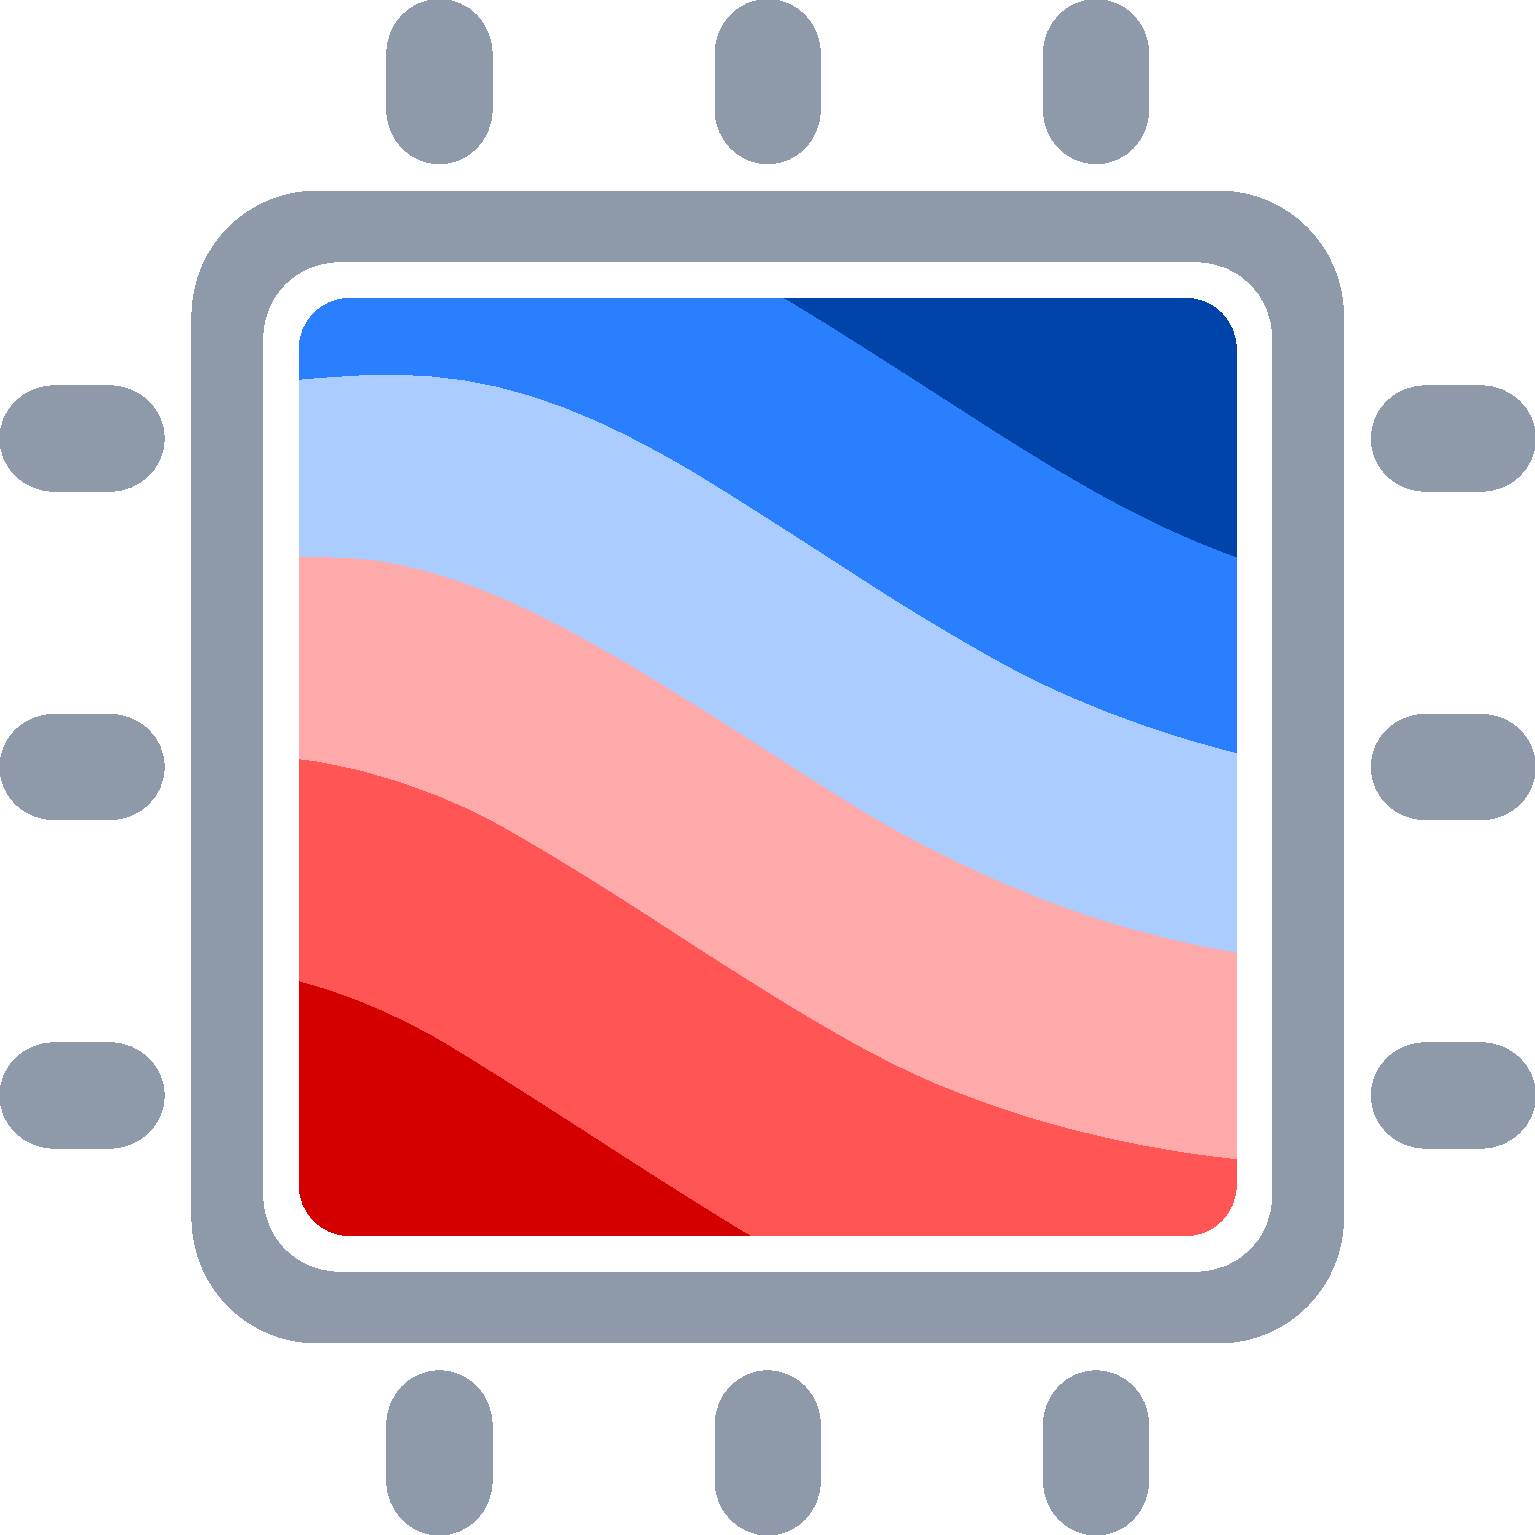
\includegraphics[height=2cm]{images/logo.pdf}
    \vspace{1cm}

    MEMORIAL PARA CONCURSO PÚBLICO

    PROFESSOR DOUTOR (RDIDP) EM MÉTODOS POTENCIAIS

    UNIVERSIDADE DE SÃO PAULO
    \vspace{4cm}

    \textbf{\LARGE \MakeUppercase{\Author{}}}
    \vspace{5cm}

    {\small
      Apresentado para concurso público de títulos e provas para cargo de

      Professor Doutor junto ao Departamento de Geofísica do

      Instituto de Astronomia, Geofísica e Ciências Atmosféricas da

      Universidade de São Paulo.
      \vspace{1cm}

      Edital ATAc-IAG/044/2022
    }
    \vfill

    \Year{}
  \end{center}
\end{titlepage}

%==============================================================================
\chapter*{Resumo}

Resumo curto.
Quem eu sou.
Principais highlights.
Sobre esse memorial (organização etc).
Meu papel no IAG.
Grande parte do texto que está na introdução do memorial antigo.

%==============================================================================
\tableofcontents

\pagestyle{fancy}
\mainmatter

%==============================================================================
\chapter{Introdução}

\begin{figure}[h]
  \HeroFigPad
  \begin{center}
    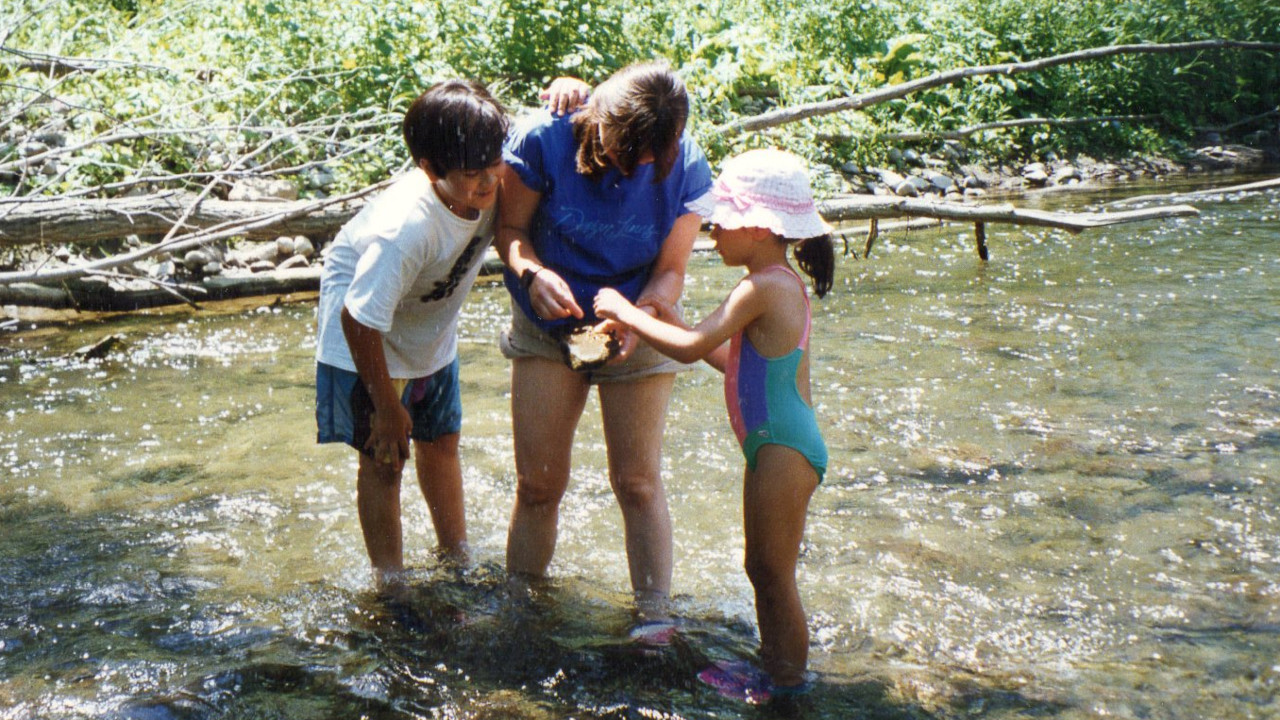
\includegraphics[width=\textwidth]{images/1997-06-ithaca-creek.jpg}
  \end{center}
  \caption{
    Minha mãe mostrando para mim e minha irmã caçula o lado inferior de uma
    pedra em um riacho, provavelmente contendo invertebrados aquáticos.
    Foto de Junho de 1997, tirada no interior do estado de Nova York, E.U.A.,
    durante o pós-doutorado de meus pais na Cornell University.
  }
  \label{fig_riacho}
\end{figure}
\begin{summarybox}[frametitle=\faInfoCircle{}\quad Informações para contato]
  \begin{fa-ul}
    \faEnvelope & email: \href{mailto:\Email}{\Email} \\
    \aiOrcid & ORCID: \href{https://orcid.org/\ORCID}{\ORCID} \\
    \aiLattes & Currículo Lattes: \href{http://lattes.cnpq.br/\Lattes}{lattes.cnpq.br/\Lattes} \\
    \aiPublonsSquare & ResearcherID: \href{https://www.webofscience.com/wos/author/rid/\ResearcherID}{\ResearcherID} \\
    \faUser & Página pessoal: \url{https://www.leouieda.com} \\
    \faUsers & Grupo de pesquisa: \url{https://www.compgeolab.org}
  \end{fa-ul}
\end{summarybox}

\section{Influências}

Sobre meus pais e meu primeiro contato com a pesquisa e ensino superior.
A ética e dedicação eles me passaram.
A oportunidade de morar no exterior.



\section{Reflexão sobre vantagens e privilégios}

Disclaimer sobre meus privilégios.
O memorial é uma reflexão das minhas conquistas.
É importante refletir também nos privilégios que me permitiram chegar onde cheguei.
Nem tudo é mérito.
Suporte familiar.
Classe média e não tive que trabalhar para apoiar meus estudos.
Escola privada.
Oportunidade de morar fora e aprender inglês.
Brasil possui ensino superior gratuito e bolsas.
Ida para o Canada foi financiada pelos meus pais.
Muitas coisas sobre o dia a dia na academia eu já sabia por ver meus pais.
Estigma contra asiáticos é relativamente baixo, pode até ser positivo nas ciências exatas.
Sorte na escolha de curso, ano de ingresso, política a favor da ciência,
professores (Mary Lilian Lourenço, Manoel Roberto Robilotta, Alan Mitchell
Durham) e mentores (Manuel, Ricardo,
Naomi, Val, Carla, Paul), vagas na hora certa, confiança e suporte para reconhecer
opoturnidades e ir atrás.

\section{Estrutura desse memorial}

Como ficou dividido. O que tem em cada parte. Links para os capítulos. Linha do
tempo.

%==============================================================================
\chapter{Formação Acadêmica}
\label{cap_formacao}

\begin{figure}[h]
  \HeroFigPad
  \begin{center}
    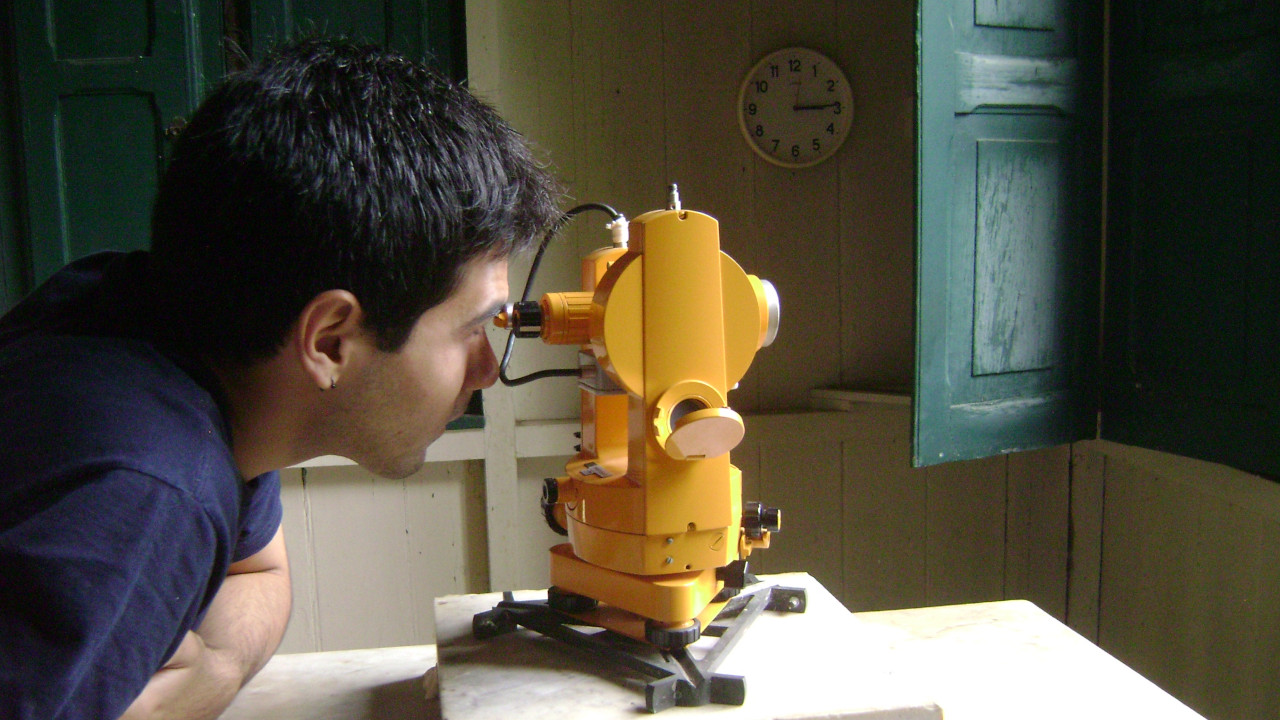
\includegraphics[width=\textwidth]{images/vassouras-geomag-observation-2012.jpg}
  \end{center}
  \caption{
    Realizando medidas da direção do campo geomagnético no observatório de
    Vassouras, RJ. A atividade foi parte de uma disciplina de instrumentação
    geofísica que cursei no mestrado do Observatório Nacional.
  }
\end{figure}
\begin{summarybox}[frametitle=\faInfoCircle{}\quad Resumo da formação acadêmica]
  \begin{datelist}
    2004--2009 & Bacharelado em Geofísica -- Universidade de São Paulo \\
    2008--2009 & \faPlane{} Intercâmbio Internacional -- York University, Canadá \\
    2010--2011 & Mestrado em Geofísica -- Observatório Nacional \\
    2011--2016 & Doutorado em Geofísica -- Observatório Nacional
  \end{datelist}
\end{summarybox}

Começa de quando ingressei na USP.
Coisas que eu aprendi, IC, TCC, campos, etc.
Turma de graduação e como isso influenciou meu pensamento.
Intercâmbio em York, geodésia, e o
Spiros Pagiatakis\footnote{\url{https://www.yorku.ca/spiros/spiros.html}}.

\section{Universidade de São Paulo}

\begin{subsummarybox}[frametitle=\faGraduationCap{}\quad Bacharelado em Geofísica]
  \begin{fa-ul}
    \faUniversity & Universidade de São Paulo \\
    \faCalendar & Fevereiro 2004 -- Novembro 2009 \\
    \faUser & Orientadora: Naomi Ussami\\
    \faInfoCircle & Trabalho de conclusão: Cálculo do tensor gradiente
    gravimétrico utilizando tesseroides \\
    \aiDoi & \DOI{10.6084/m9.figshare.963547}
  \end{fa-ul}
\end{subsummarybox}

\section{York University}

\begin{subsummarybox}[frametitle=\faPlane{}\quad Intercâmbio internacional]
  \begin{fa-ul}
    \faUniversity & York University, Canadá\\
    \faCalendar & Agosto 2008 -- Maio 2009\\
    \faInfoCircle & Disciplinas de geodésia e posicionamento no curso de
    Engenharia Geomática.
  \end{fa-ul}
\end{subsummarybox}

Como surgiu a oportunidade.
Processo competitivo contra alunos de toda a universidade.
Ter o inglês fluente me deu muita vantagem.
Apoio da Naomi e do Departamento pagando minha passagem.
Aprender geodésia era o alvo.
Surpresa que o curso não existia mais.

Aprendi sobre sistemas de coordenadas que foi usado diretamente no meu TCC.
Geodésia física com o Spiros foi a base para quase todo meu trabalho hoje em dia.
Aprendi como usar um gravímetro e construir redes gravimétricas.
Toda a teoria base da inversão, incluindo experiência prática na construção e
solução numérica de problemas inversos.

Descobri o Software Carpentry e aprendi sobre controle versão, testes unitários,
Make, programação defensiva, e outros.
Apliquei imediatamente.
São úteis até hoje. Tudo que eu produzo está sob controle de versão.
Meu ensino de programação é baseado nessa experiência (ver formação abaixo).
Saber subversion me permitiu fazer a transição do GMT.

Amizades para toda a vida e intercâmbio cultural com canadenses, europeus,
turcos, asiáticos que teria pouco contato em outras circunstâncias.


\section{Observatório Nacional}

\begin{subsummarybox}[frametitle=\faGraduationCap{}\quad Mestrado em Geofísica]
  \begin{fa-ul}
    \faUniversity & Observatório Nacional \\
    \faCalendar & Fevereiro de 2010 -- Outubro de 2011 \\
    \faUser & Orientadora:  Valéria C. F. Barbosa\\
    \faInfoCircle & Dissertação: Robust 3D gravity gradient inversion by
    planting anomalous densities\\
    \aiDoi & \DOI{10.6084/m9.figshare.16882300}
  \end{fa-ul}
\end{subsummarybox}
\begin{subsummarybox}[frametitle=\faGraduationCap{}\quad Doutorado em Geofísica]
  \begin{fa-ul}
    \faUniversity & Observatório Nacional \\
    \faCalendar & Novembro de 2011 -- Abril de 2016 \\
    \faUser & Orientadora:  Valéria C. F. Barbosa\\
    \faInfoCircle & Tese Modelagem direta e inversão de campos gravitacionais em
    coordenadas esféricas \\
    \aiDoi & \DOI{10.6084/m9.figshare.16883689} \\
    \faTrophy & Ganhador do Prêmio SBGf de Melhor Tese de Doutorado (2015--2017)\footnotemark
  \end{fa-ul}
\end{subsummarybox}
\footnotetext{\url{https://sbgf.org.br/premiacoes/}}

Criação do pinga.
Trabalhos com o biroca.
Cursos que foram críticos.
Participação em congressos.
Liberdade que a Val me deu para escolher temas.
Aprendendo sobre programação e ciência aberta.
Aprendendo sobre criação de websites e tecnologias de web.
Scipy e conhecendo o povo do SimPEG.
Disciplinas da pós de calor da terra, inversão e gravmag.
Começando o Fatiando para auxiliar na minha tese.
Ter a base do Fatiando me permitiu terminar tudo a tempo, tanto a tese quanto
as aulas na UERJ.
Ter a base da York e USP me permitiram começar a trabalhar no meu projeto imediatamente.
Por isso que eu consegui inovar direto no mestrado.
Valéria me deu muitas oportunidades de congresso que foram cruciais e me ajudaram a fazer contatos internacionais.
Ter o inglês fluente me facilitou muito a vida.
Ambiente na sala da pós graduação de colaboração.
Intercâmbio de ideias com diversas áreas da geofísica e da astronomia.
Aprendi muito de sísmica ajudando o Saulo a rodar o Madagascar, por exemplo.
Viagem para Trieste para trabalhar com a Carla.


\section{Formação complementar}

Esses foram os cursos que deram algum tipo de habilitação especial.

\begin{subsummarybox}[frametitle=\faGraduationCap{}\quad The Carpentries Instructor Training]
  \begin{fa-ul}
    \faUniversity & \href{https://carpentries.org/}{The Carpentries} \\
    \faCalendar & 9--10 de Julho de 2018\\
    \faInfoCircle & Habilitação para organizar e ministrar os cursos
    \textit{Software Carpentry}, \textit{Data Carpentry} e
    \textit{Library Carpentry}, incluindo treinamento em pedagogia e práticas
    de ensino de programação e ciência de dados\footnotemark{}
  \end{fa-ul}
\end{subsummarybox}
\footnotetext{\url{https://carpentries.org/instructors/\#leouieda}}

Falar sobre a iniciativa de treinamento de instrutores.
Fiz uma versão online em 2017 mas não terminei.
Porém, usei o modelo online deles (Zoom + Google Docs + Breakout Rooms) nas
minhas aulas durante a pandemia.
Fiz o curso presencial no Scipy.
Completei o curso fazer uma aula e contribuindo para o material didático\footnote{colocar link do pull request}.

\begin{subsummarybox}[frametitle=\faGraduationCap{}\quad Postgraduate Certificate Academic Practice]
  \begin{fa-ul}
    \faUniversity & Universidade de Liverpool \\
    \faCalendar & Novembro de 2020 -- Maio de 2022 \\
    \faInfoCircle & Curso de pedagogia no ensino superior que me confere o
    título de \textit{Fellow of the Higher Education Academy}\footnotemark{}
    (número de referência PR242069)
  \end{fa-ul}
\end{subsummarybox}
\footnotetext{\url{https://www.advance-he.ac.uk/fellowship/fellowship}}

Curso PGCAP para preparo pedagógico de novos docentes.
Primeira parte era teórica com exercícios e reflexões.
Peer obervation (observação por pares) foi muito bom.
Uma pessoa observa uma das aulas e dá feedback depois.
Modelo efetivo.
Tem evidência de que isso funciona muito bem e é empregado em contextos de
ensino médio e fundamental (citar artigos).
Estudo sugerem que funciona bem no ensino superior, principalmente se for
positivo e para melhoramento e não julgamento.
Produção de material audio visual.
Colocar a filosofia de ensino no papel e fazer um vídeo.
https://youtu.be/ABYEIuvXqy4

Oportunidade de estudar teoria pedagógica aplicada à geociências e computação.
Listar exemplos de trabalhos influêntes.
Fazer isso de forma organizada ajudou e compilar num portfólio público ajuda
no acesso e aumenta a utilidade do curso.

Criei o portfólio de atividades e um projeto de revisão para a segunda parte.
\url{https://www.leouieda.com/pgcap}

%==============================================================================
\chapter{Atuação Profissional}
\label{cap_atuacao}

\begin{figure}[h]
  \HeroFigPad
  \begin{center}
    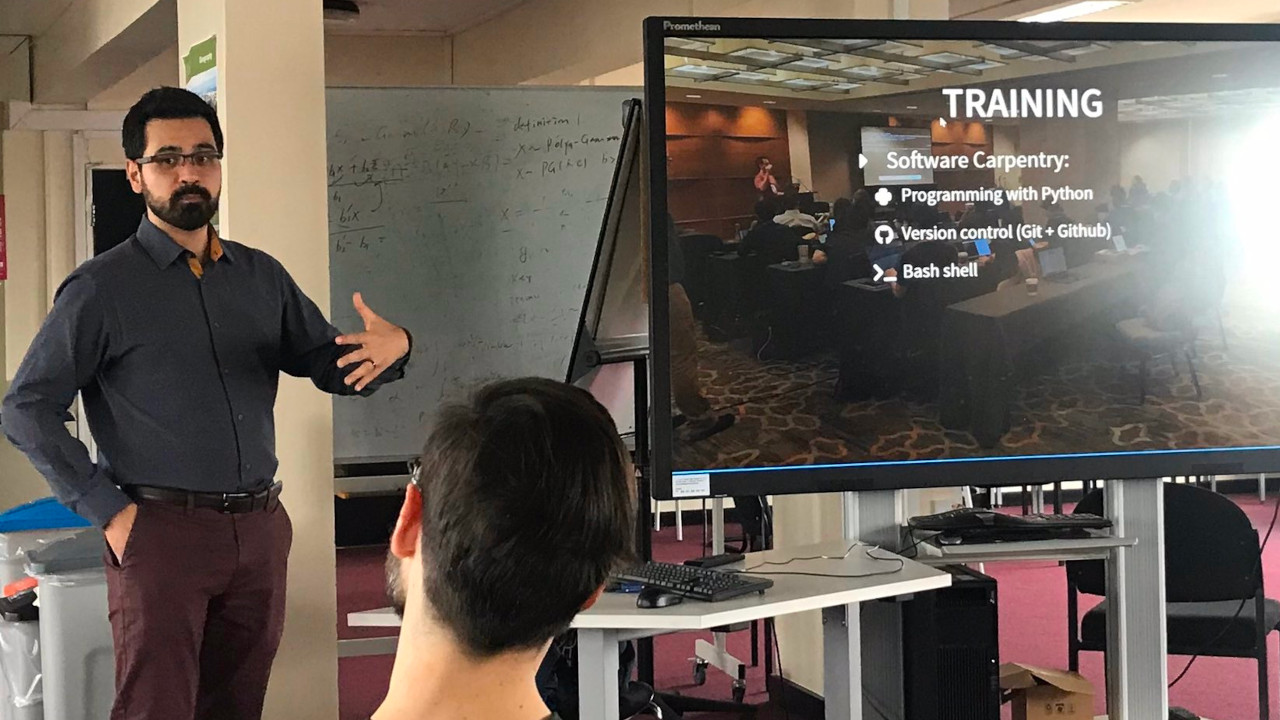
\includegraphics[width=\textwidth]{images/liverpool-gdsl.jpg}
  \end{center}
  \caption{
    Foto de uma apresentação que fiz para o \textit{Geographic Data Science
    Lab} da Universidade de Liverpool em Março de 2020. O propósito da palestra
    era me apresentar para o grupo pouco após minha chegada em Liverpool.
  }
\end{figure}
\begin{summarybox}[frametitle=\faInfoCircle{}\quad Resumo da atuação profissional]
  \begin{datelist}
    2014--2018 & Professor Assistente -- \UERJ \\
    2017--2019 & Pesquisador Visitante -- \UHM, E.U.A. \\
    2019--atual & Lecturer (\textit{Professor Doutor}) -- University of Liverpool, Reino Unido
  \end{datelist}
\end{summarybox}

\section{\UERJ}

\begin{subsummarybox}[frametitle=\faUniversity{}\quad Vínculo institucional]
  \begin{fa-ul}
    \faUser & Professor Assistente \\
    \faMapMarker & Departamento de Geologia Aplicada -- Faculdade de Geologia \\
    \faCalendar & Fevereiro 2014 -- Janeiro 2018 \\
    \faTrophy & Paraninfo da turma XXX
  \end{fa-ul}
\end{subsummarybox}
\begin{subsummarybox}[frametitle=\faList{}\quad Atividades institucionais]
  \begin{datelist}
    2014--2017 & Coordenador: Laboratório de Geofísica de Exploração (LAGEX)\\
    2014--2017 & Coordenador: Projeto Qualitec para contratação de um bolsista de nível superior para atuar no LAGEX\\
    2015--2017 & \textit{Faculty Advisor}: Capítulo Estudantil da Society of
    Exploration Geophysicists (\textit{UERJ Geophysical Society}) \\
    201X & ELEIÇÃO
  \end{datelist}
\end{subsummarybox}

SEG Chapter\footnote{\url{https://seg.org/Education/Student/Student-Chapters/Student-Chapter-Details/student-chapter-listing-details/scID/000000440245}}

Coordenação do LAGEX.

QUALITEC. Victor e Gabriela.

Capítulo SEG.

\url{https://seg.org/Education/Student/Student-Chapters/Student-Chapter-Details/student-chapter-listing-details/scID/000000440245}

Eleição


\section{\UHM}

\begin{subsummarybox}[frametitle=\faUniversity{}\quad Vínculo institucional]
  \begin{fa-ul}
    \faUser & Pesquisador Visitante \\
    \faMapMarker & Department of Earth Sciences -- School of Ocean and Earth Science and Technology\\
    \faCalendar & Fevereiro 2017 -- Agosto 2019
  \end{fa-ul}
\end{subsummarybox}



\section{University of Liverpool}

\begin{subsummarybox}[frametitle=\faUniversity{}\quad Vínculo institucional]
  \begin{fa-ul}
    \faUser & Lecturer (\textit{equivalente a Professor Doutor})\\
    \faMapMarker & Department of Earth, Ocean and Ecological Sciences -- School of Environmental Sciences \\
    \faCalendar & Agosto 2019 -- Presente
  \end{fa-ul}
\end{subsummarybox}
\begin{subsummarybox}[frametitle=\faList{}\quad Atividades institucionais]
  \begin{datelist}
    2020--2022 & Comissão para avaliação do website do departamento\\
    2020--atual & Early Career Academic (ECA) Representative -- Earth Sciences\\
    2022--atual & Coordenador de curso: Bacharelado em Geofísica e Mestrado em Geologia e Geofísica
  \end{datelist}
\end{subsummarybox}


\section{Atuação na Comunidade Científica}

\begin{subsummarybox}[frametitle=\faList{}\quad Resumo das atividades]
  \begin{datelist}
    2019--2022 & \href{https://joss.theoj.org/}{Journal of Open Source Software}
    (ISSN 2475-9066): Topic Editor \\
    2019--2022 & \href{https://eartharxiv.org/}{EarthArXiv}: Advisory Council Member \\
    2022--atual & \href{https://softwareunderground.org}{Software Underground}:
             Board Member \\
    2022--atual & \href{https://www.pyopensci.org/}{pyOpenSci}:
             Advisory Committee Member
  \end{datelist}
\end{subsummarybox}

JOSS\footnote{\url{https://joss.theoj.org/about\#editors\_emeritus}}

Software Underground\footnote{\url{https://softwareunderground.org/board}}

EarthArXiv\footnote{\url{https://eartharxiv.github.io/AdvisoryCouncil.html}}

pyOpenSci\footnote{\url{https://www.pyopensci.org/our-community/\#pyopensci-working-advisory-committee}}

Revisor de periódicos\footnote{\url{https://www.webofscience.com/wos/author/rid/\ResearcherID}}:
Geophysical Journal International,
Geophysics,
Journal of Geodesy,
Pure and Applied Geophysics,
Journal of Applied Geophysics,
Geophysical Prospecting,
Central European Journal of Geosciences,
Computers and Geosciences
e
Journal of Open Source Software.

Bancas:
2022External PhD thesis examiner (Peter Haas), Christian-Albrechts-Universität zu Kiel.
2022Internal PhD thesis examiner (Yael Annemiek Engbers), University of Liverpool.
2016Internal MSc dissertation examiner (Natacha Medeiros Rocha), Universidade do Estado do Rio
de Janeiro.
Organização de eventos:

%==============================================================================
\chapter{Ciência Aberta}
\label{cap_cienciaaberta}

\begin{figure}[h]
  \HeroFigPad
  \begin{center}
    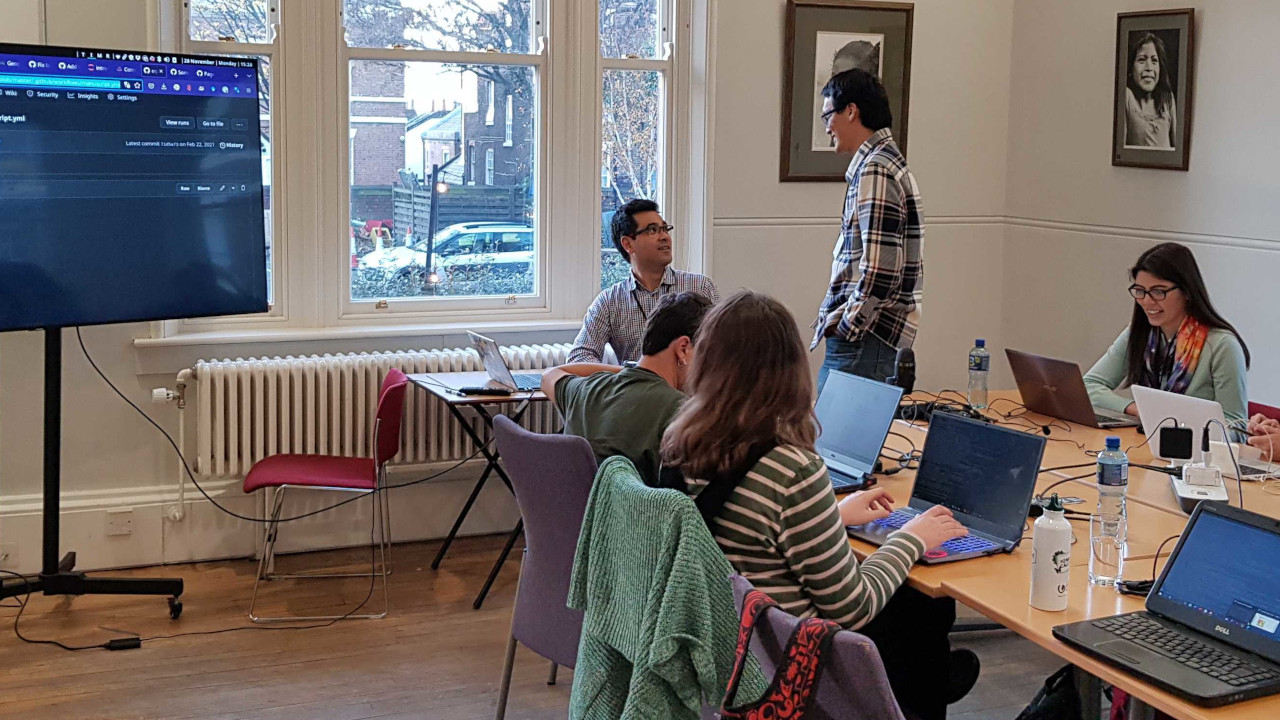
\includegraphics[width=\textwidth]{images/geopluscode.jpg}
  \end{center}
  \caption{
    Foto do evento \textit{Geo+Code UK} que organizei com meu financiamento
    do \href{https://software.ac.uk/}{Software Sustainability Institute} em
    Novembro de 2022. Durante o evento, demos início à criação de um
    livro texto digital sobre geofísica aplicada que será desenvolvido
    conjuntamente por educadores de diversas instituições do Reino Unido e
    Irlanda.
  }
\end{figure}
\begin{summarybox}[frametitle=\faInfoCircle{}\quad Portfólio de produção em ciência aberta]
  \begin{fa-ul}
    \faGithub & GitHub: \url{https://github.com/leouieda}
      (código, material didático) \\
    \aiFigshare & figshare: \url{https://figshare.com/authors/Leonardo\_Uieda/97471}
      (dados, apresentações, material suplementar) \\
    \aiImpactstory & Impactstory: \url{https://impactstory.org/u/0000-0001-6123-9515}
      (análise contextual da produção aberta) \\
    \faYoutube & YouTube: \url{https://youtube.com/LeonardoUieda}
      (palestras, tutoriais, aulas)
  \end{fa-ul}
\end{summarybox}

Como eu abordo a pesquisa e ensino.
Computacional primeiro.
Reprodutibilidade.
Dados abertos e FAIR principles.

Os princípios de dados FAIR (\textit{Findable, Accessible, Interoperable,
Reusable}) foram estabelecidos em \citet{Wilkinson2016}.
SSI.
EarthArXiv.
Software Underground.
JOSS.
pyOpenSci.

\begin{subsummarybox}[frametitle=\faInfoCircle{}\quad Apresentações sobre ciência aberta]
  \begin{paperlist}
    2022 &
      \Me.
      Getting started with Open Science,
      \emph{SPIN SPIN-ITN: Seismological Parameters and Instrumentation}.
      \GitHub{leouieda/2022-05-06-spin-open-science}.
      \\
    2021 &
      \Me, \Santiago.
      Python-based workflows for small-to-medium sized data: what works, what
      doesn't, and what can be improved,
      \emph{AGU 2021}. \GitHub{compgeolab/agu2021}.
      \\
    ~ &
      \Me.
      Academia e software livre: Desafios e oportunidades no Brasil e no exterior,
      \emph{National Observatory's SEG and EAGE Student Chapter},
      Rio de Janeiro, Brazil.
      \GitHub{leouieda/2021-07-22-on}.
      \YouTube{r2x-DN6laj8}.
      \\
    2020 &
      \Me.
      Geophysical research powered by open-source,
      \emph{Christian Albrechts Universität zu Kiel},
      Kiel, Germany.
      \GitHub{leouieda/2020-07-01-kiel}.
      \\
    ~ &
      \Me.
      Geophysical research powered by open-source,
      \emph{Departamento de Geofísica, IAG, Universidade de São Paulo}.
      \GitHub{leouieda/2020-06-18-usp}.
      \YouTube{VqI8BX1Yg54}.
      \\
    ~ &
      \Me.
      Geophysical research powered by open-source,
      \emph{Technische Universität Bergakademie Freiberg}.
      \GitHub{leouieda/2020-06-04-freiberg}.
      \\
    ~ &
      \Me.
      Geophysical research powered by open-source,
      \emph{Geographic Data Science Lab, University of Liverpool}.
      \GitHub{leouieda/liverpool-gdsl-2020}.
      \\
    2019 &
      \Me.
      Building the foundations for open-source geophysics,
      \emph{University of Liverpool}.
      \DOI{10.6084/m9.figshare.10255832}.
      \\
    2017 &
      \Me, \Paul.
      Nurturing reliable and robust open-source scientific software,
      \emph{AGU Fall Meeting}.
      \YouTube{0GO4ZZ5Ry6M}.
  \end{paperlist}
\end{subsummarybox}

Materiais de ensino aberto. Citar uns artigos aqui.

Listar aqui algumas das produções que são meio aleatórias, tipo o curso de
ciência aberta.

\section{Software livre}

Meu primeiro contato com a ciência aberta foi pesquisando sobre os sistemas
GNU/Linux que era operados pelo IAG.
Os princípios de software livre formaram o arcabouço da minha abordagem
científica.
Os códigos que possibilitam minhas atividades de pesquisa e ensino.

Apresento abaixo um resumo da minha produção relacionada a software livre,
seguido de contextualizações para cada um projetos relacionados a esse tema.

\subsection{Tesseroids}

\begin{summarybox}[frametitle=\faInfoCircle{}\quad Informações sobre o projeto]
  \begin{fa-ul}
    \faLink & Página principal: \url{https://tesseroids.leouieda.com}
    \\
    \faGithub & Código: \url{https://github.com/leouieda/tesseroids}
    \\
    \faGavel & Licença: \href{https://github.com/leouieda/tesseroids/blob/master/LICENSE.txt}{BSD 3-clause}
    \\
    \aiGoogleScholarSquare & 146 citações no \href{https://scholar.google.com/citations?view\_op=view\_citation\&hl=en\&user=qfmPrUEAAAAJ\&citation\_for\_view=qfmPrUEAAAAJ:AXPGKjj\_ei8C}{Google Scholar}\footnotemark{} (acessado em 27/12/2022)
  \end{fa-ul}
\end{summarybox}
\footnotetext{Citações ao trabalho \citet{Uieda2016}.}
\begin{subsummarybox}[frametitle=\faFilePdf{}\quad Artigos publicados]
  \begin{paperlist}
    2016 &
      \Me, \Val, \Carla.
      Tesseroids: Forward modeling gravitational fields in spherical coordinates,
      \emph{Geophysics}, \DOI{10.1190/geo2015-0204.1}.
      \GitHub{pinga-lab/paper-tesseroids}.
  \end{paperlist}
\end{subsummarybox}

Figura com o logo do Tesseroids.
Primeiro projeto de software.
Como foi abordado.
Começou em C.
Passei para Python.
Voltei para C com a Carla em Trieste.
Uso do software e citações.

\subsection{Fatiando a Terra}

\begin{summarybox}[frametitle=\faInfoCircle{}\quad Informações sobre o projeto]
  \begin{fa-ul}
    \faLink & Página principal: \url{https://www.fatiando.org}
    \\
    \faGithub & Código: \url{https://github.com/fatiando}
    \\
    \faGavel & Licença: \href{https://opensource.org/licenses/BSD-3-Clause}{BSD 3-clause}
    \\
    \aiGoogleScholarSquare & 119 citações no \href{https://scholar.google.com/citations?user=qfmPrUEAAAAJ}{Google Scholar}\footnotemark{} (acessado em 27/12/2022)
  \end{fa-ul}
\end{summarybox}
\footnotetext{Total de citações aos trabalhos \citet{Uieda2013}, \citet{Uieda2018} e \citet{Uieda2020}.}
\begin{subsummarybox}[frametitle=\faFilePdf{}\quad Artigos publicados]
  \begin{paperlist}
    2020 &
      \Me, \Santiago, \Remi, \Hugo, \MattTurk, \Shapero, \Anderson, \Leeman.
      Pooch: A friend to fetch your data files.
      \emph{Journal of Open Source Software}.
      \DOI{10.21105/joss.01943}.
      \GitHub{fatiando/pooch}.
      \\
    2018 &
      \Me. Verde: Processing and gridding spatial data using Green's functions.
      \emph{Journal of Open Source Software}.
      \DOI{10.21105/joss.00957}.
      \GitHub{fatiando/verde}.
  \end{paperlist}
\end{subsummarybox}
\begin{subsummarybox}[frametitle=\faFile{}\quad Trabalhos completos em anais de eventos]
  \begin{paperlist}
    2013 &
      \Me, \Bi, \Val.
      Modeling the Earth with Fatiando a Terra,
      \emph{Proceedings of the 12th Python in Science Conference}.
      \DOI{10.25080/Majora-8b375195-010}.
      \GitHub{leouieda/scipy2013}.
  \end{paperlist}
\end{subsummarybox}
\begin{subsummarybox}[frametitle=\faInfoCircle{}\quad Apresentações]
  \begin{paperlist}
  \end{paperlist}
\end{subsummarybox}

Figura com o banner do Fatiando.

Como surgiu, o grupo no IAG, aprendendo subversion.
Colocar links para os commits.
Desenvolvimento na pós e o curso do IAG.
Uso na minha dissertação e tese e matérias da UERJ.

Entrada do Santiago como um marco.

Conhecendo o pessoal do SimPEG/PyGIMLi/GemPy e formação do Software Underground.
Overlap.
Reestruturação do Fatiando (link pro meu post).

Novos pacotes.
Mais participação consistente da comunidade (Agustina, Mariana, Lu, Matt).

Pooch como um caso de sucesso.
Como surgiu.
Podcast sobre o Pooch.
Uso em vários pacotes.

\subsection{Generic Mapping Tools}

\begin{summarybox}[frametitle=\faInfoCircle{}\quad Informações sobre o projeto GMT]
  \begin{fa-ul}
    \faLink & Página principal: \url{https://www.generic-mapping-tools.org}
    \\
    \faGithub & Código: \url{https://github.com/GenericMappingTools}
    \\
    \faGavel & Licença: \href{https://opensource.org/licenses/LGPL-3.0}{GNU LGPL}
    \\
    \aiGoogleScholarSquare & 934 citações no \href{https://scholar.google.com/citations?view\_op=view\_citation\&hl=en\&user=qfmPrUEAAAAJ\&citation\_for\_view=qfmPrUEAAAAJ:hkOj\_22Ku90C}{Google Scholar}\footnotemark{} (acessado em 27/12/2022)
  \end{fa-ul}
\end{summarybox}
\footnotetext{Citações ao trabalho \citet{Wessel2019}.}
\begin{summarybox}[frametitle=\faInfoCircle{}\quad Informações sobre o projeto PyGMT]
  \begin{fa-ul}
    \faLink & Página principal: \url{https://www.pygmt.org}
    \\
    \faGithub & Código: \url{https://github.com/GenericMappingTools/pygmt}
    \\
    \faGavel & Licença: \href{https://github.com/GenericMappingTools/pygmt/blob/main/LICENSE.txt}{BSD 3-clause}
    \\
    \aiGoogleScholarSquare & 43 citações no \href{https://scholar.google.com/citations?view\_op=view\_citation\&hl=en\&user=qfmPrUEAAAAJ\&citation\_for\_view=qfmPrUEAAAAJ:-\_dYPAW6P2MC}{Google Scholar}\footnotemark{} (acessado em 27/12/2022)
  \end{fa-ul}
\end{summarybox}
\footnotetext{Citações ao trabalho \citet{Uieda2022}.}
\begin{subsummarybox}[frametitle=\faFilePdf{}\quad Artigos publicados]
  \begin{paperlist}
    2019 &
      \Paul, \Joaquim, \Me, \Remko, \Florian, \Walter, \Dongdong.
      The Generic Mapping Tools, Version 6.
      \emph{Geochemistry, Geophysics, Geosystems}.
      \DOI{10.1029/2019GC008515}.
  \end{paperlist}
\end{subsummarybox}
\begin{subsummarybox}[frametitle=\faInfoCircle{}\quad Apresentações]
  \begin{paperlist}
  \end{paperlist}
\end{subsummarybox}

Como me envolvi com o GMT.
Criação do PyGMT.
Comunidade que surgiu ao entrono.
Projeto da NSF e o Max.
\citep{Wessel2019}.

Summits do GMT.
Transição para o GitHub.
Website e documentação automatizados.
Abertura no modelo de desenvolvimento == maior participação tanto com exemplos,
discussões e até código.

\subsection{xlandsat}

\begin{summarybox}[frametitle=\faInfoCircle{}\quad Informações sobre o projeto]
  \begin{fa-ul}
    \faLink & Página principal: \url{https://compgeolab.org/xlandsat}
    \\
    \faGithub & Código: \url{https://github.com/compgeolab/xlandsat}
    \\
    \faGavel & Licença: \href{https://github.com/compgeolab/xlandsat/blob/main/LICENSE.txt}{MIT}
  \end{fa-ul}
\end{summarybox}

Último pacote a ser criado no âmbito do CompGeoLab.
Uso nas aulas e também para divulgação científica.
Por exemplo o Mauna Loa.
Colocar figura bonita e link para o meu blog.


\section{Dados abertos}

Na verdade melhor falar em FAIR.
Por que usar CC-BY ou CC0 é importante.

Compilação de dados do Fatiando.
Compilação da Austrália.


\section{Reprodutibilidade}

Alguma coisa sobre o Clarebout e Madagascar como influências iniciais.
Por que isso importa.
Lorena Barba.

Publicação de todo o código no GitHub e figshare desde meu primeiro artigo em
2012.
O approach atual de colocar o máximo possível nos pacotes durante o
desenvolvimento da pesquisa.
Exemplo da EQLGB.

\section{Acesso livre}

JOSS e EarthArXiv.


\section{Recursos educacionais abertos}

\begin{subsummarybox}[frametitle=\faFilePdf{}\quad Artigos publicados em revistas]
  \begin{paperlist}
    2017 &
      \Me.
      Step-by-step NMO correction,
      \emph{The Leading Edge},
      \DOI{10.1190/tle36020179.1}.
      \GitHub{pinga-lab/nmo-tutorial}.
      \\
    2014 &
      \Me, \Bi, \Val.
      Geophysical tutorial: Euler deconvolution of potential-field data,
      \emph{The Leading Edge},
      \DOI{10.1190/tle33040448.1}.
      \GitHub{pinga-lab/paper-tle-euler-tutorial}.
  \end{paperlist}
\end{subsummarybox}
\begin{subsummarybox}[frametitle=\faInfoCircle{}\quad Recursos educacionais]
  \begin{paperlist}
    2021 &
      \Me. A quick introduction to machine learning.
      \GitHub{leouieda/ml-intro}.
      \\
    2020 &
      \Me. Introduction to lithosphere dynamics.
      \GitHub{leouieda/lithosphere}.
      \\
    2020 &
      \Me. Introduction to remote sensing.
      \GitHub{leouieda/remote-sensing}.
      \\
    2015 &
      \Me. Matemática Especial 1: Introdução à computação e métodos numéricos.
      \GitHub{mat-esp/about}.
      \\
    2015 &
      \Me. Geofísica 2: Sismologia e métodos eletromagnéticos.
      \GitHub{leouieda/geofisica2}.
      \\
    2015 &
      \Me. Geofísica 1: Gravimetria e magnetometria.
      \GitHub{leouieda/geofisica1}.
      \\
    2014 &
      \Bi, \Me. Tópicos de inversão em geofísica.
      \DOI{10.6084/m9.figshare.1192984}.
      \GitHub{pinga-lab/inverse-problems}.
  \end{paperlist}
\end{subsummarybox}
\begin{subsummarybox}[frametitle=\faInfoCircle{}\quad Vídeos]
  \begin{paperlist}
    2022 & A geophysical tour of mid-ocean ridges. \YouTube{NzJmRlJCNbQ}
      \\
    2022 & Anatomy of a PyGMT figure. \YouTube{96\_reU\_yh5I}
      \\
    2021 & Downloading Landsat 8 images from USGS EarthExplorer. \YouTube{Wn\_G4fvitV8}
      \\
    2021 & Searching on Google for openly licensed images. \YouTube{ISu51NB5Z28}
      \\
    2020 & From scattered data to gridded products using Verde. \YouTube{-xZdNdvzm3E}
  \end{paperlist}
\end{subsummarybox}


https://www.unesco.org/en/open-educational-resources

Tutoriais da TLE.
Material de geofísica 1 e 2.
Material de Liverpool.

Geophysics Library e Geo+Code.



%==============================================================================
\chapter{Linhas de Pesquisa}
\label{cap_pesquisa}

\begin{figure}[h]
  \HeroFigPad
  \begin{center}
    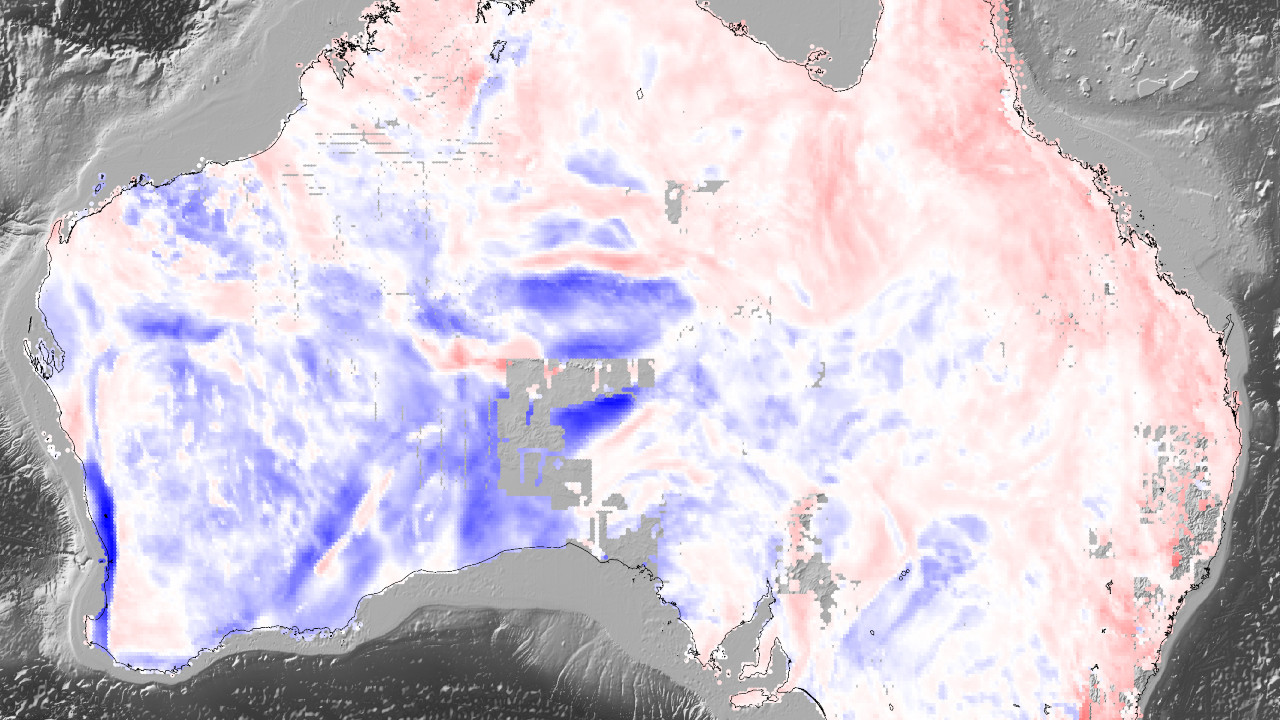
\includegraphics[width=\textwidth]{images/australia-ground-gravity-disturbance.jpg}
  \end{center}
  \caption{
    Compilação de dados terrestres de distúrbio da gravidade da Austrália.
    Distribuídos originalmente por \citet{Wynne2018}. Compilados e padronizados
    por \citet{Uieda2021}.
  }
\end{figure}
\begin{summarybox}[frametitle=\faInfoCircle{}\quad Resumo das atividades]
  \begin{fa-ul}
    \faSearchDollar & Projetos financiados pelas agências: National Science
      Foundation (E.U.A.), Royal Society (Reino Unido) e Software Sustainability
      Institute (Reino Unido)\\
    \faUserGraduate & Orientações concluídas: 11 de graduação, 1 de mestrado, 1
      co-orientação de doutorado \\
    \faUser & Orientações em andamento: 1 de graduação, 1 de doutorado, 1
      co-orientação de doutorado \\
    \faFilePdf & 13 artigos publicados em revistas indexadas, 3 em outras
    revistas, 11 trabalhos completos em anais de eventos\footnotemark[1] \\
    \faComment & 38 apresentações de trabalho, sendo 13 dessas convidadas\footnotemark[1] \\
    \aiGoogleScholarSquare & 1736 citações no \href{https://scholar.google.com/citations?user=qfmPrUEAAAAJ}{Google Scholar} e 959 no \href{https://www.webofscience.com/wos/author/record/1766625}{Web of Science} (acessados em 27/12/2022)
  \end{fa-ul}
\end{summarybox}
\footnotetext[1]{O número de total trabalhos e apresentações pode ser diferente
das quantidades listadas abaixo. Alguns trabalhos e apresentações estão
listados em outras áreas de atuação (e.g., capítulo \ref{cap_cienciaaberta}) ou
pertencem a mais de uma linha de pesquisa.}

Esse capítulo é uma reflexão da minha trajetória de pesquisa, da graduação até
minha posição atual na Universidade de Liverpool.
Ciência de impacto.
Bem social.
Grandes problemas e questões.

É preciso enfatizar que nem todos os artigos, projetos financiados e
apresentações contados acima estão listados nas seções abaixo.
Alguns estão listados no capítulo \ref{cap_cienciaaberta}.

PINGA e CompGeoLab.

\section{Modelagem direta de campos gravitacionais em coordenadas esféricas}

Tesseroids.
Ajuda da Wild-Pfeiffer.
TCC.
Carla.
Trieste.
Discretização adaptative.
Software.
Utilização para fazer os grids do GOCE.

Projeto inicial do Santiago.
Contato com Guangdong depois de uma revisão.
Mustafa começou com a parte elipsoidal.

\begin{subsummarybox}[frametitle=\faFilePdf{}\quad Artigos publicados]
  \begin{paperlist}
    2019 & \Santiago, \Agustina, \Gimenez, \Me.
      Gravitational field calculation in spherical coordinates using variable
      densities in depth.
      \emph{Geophysical Journal International}.
      \DOI{10.1093/gji/ggz277}.
      \GitHub{pinga-lab/tesseroid-variable-density}.
      \Preprint{10.31223/osf.io/3548g}.
      \Data{10.6084/m9.figshare.8239622}.
      \\
    ~ & \Guangdong, \Bo, \Me, \JLiu, \MKaban, \LChen, \RGuo.
      Efficient 3D large-scale forward-modeling and inversion of gravitational fields in
      spherical coordinates with application to lunar mascons.
      \emph{Journal of Geophysical Research: Solid Earth}.
      \DOI{10.1029/2019jb017691}.
      \Preprint{10.31223/osf.io/dzf9j}.
      \Data{10.6084/m9.figshare.7300523}.
      \\
    2016 & \Me, \Val, \Carla.
      Tesseroids: Forward modeling gravitational fields in spherical coordinates,
      \emph{Geophysics}, \DOI{10.1190/geo2015-0204.1}.
      \GitHub{pinga-lab/paper-tesseroids}.
  \end{paperlist}
\end{subsummarybox}
\begin{subsummarybox}[frametitle=\faFile{}\quad Trabalhos completos em anais de eventos]
  \begin{paperlist}
    2011 & \Me, \Everton, \Carla, \Eder.
      Optimal forward calculation method of the Marussi tensor due to a geologic
      structure at GOCE height,
      \emph{Proceedings of the 4th International GOCE User Workshop}.
      \DOI{10.6084/m9.figshare.92624}.
      \GitHub{leouieda/goce2011}.
  \end{paperlist}
\end{subsummarybox}
\begin{subsummarybox}[frametitle=\faInfoCircle{}\quad Outras apresentações]
  \begin{paperlist}
    2010 & \Me, \Naomi, \Carla.
      Computation of the gravity gradient tensor due to topographic masses
      using tesseroids,
      \emph{AGU Meeting of the Americas},
      Foz do Iguaçu, Brazil.
      \DOI{10.6084/m9.figshare.156858}
      \\
    2008 & \Me, \Naomi.
      Utilização de tesseróides na modelagem de dados de gradiometria
      gravimétrica,
      \emph{XIII Simpósio de Iniciação Científica do IAG-USP},
      São Paulo, Brazil.
      \DOI{10.6084/m9.figshare.4779760}
  \end{paperlist}
\end{subsummarybox}



\section{Inversão 3D em métodos potenciais}

Seed e trabalhos do Dio.
Inversão do Guangdong.

\begin{subsummarybox}[frametitle=\faFilePdf{}\quad Artigos publicados]
  \begin{paperlist}
    2019 &
      \Guangdong, \Bo, \Me, \JLiu, \MKaban, \LChen, \RGuo.
      Efficient 3D large-scale forward-modeling and inversion of gravitational fields in
      spherical coordinates with application to lunar mascons.
      \emph{Journal of Geophysical Research: Solid Earth}.
      \DOI{10.1029/2019jb017691}.
      \Preprint{10.31223/osf.io/dzf9j}.
      \Data{10.6084/m9.figshare.7300523}.
      \\
    2016 &
      \Dio, \Me, \Val.
      How two gravity-gradient inversion methods can be used to reveal different
      geologic features of ore deposit - A case study from the Quadrilátero
      Ferrífero (Brazil),
      \emph{Journal of Applied Geophysics},
      \DOI{10.1016/j.jappgeo.2016.04.011}.
      \\
    2014 &
      \Dio, \Me, \Val.
      Imaging iron ore from the Quadrilátero Ferrífero (Brazil) using geophysical
      inversion and drill hole data,
      \emph{Ore Geology Reviews},
      \DOI{10.1016/j.oregeorev.2014.02.011}.
      \\
    2012 &
      \Me, \Val.
      Robust 3D gravity gradient inversion by planting anomalous densities,
      \emph{Geophysics},
      \DOI{10.1190/geo2011-0388.1}.
      \GitHub{pinga-lab/paper-planting-densities}.
      \Data{10.6084/m9.figshare.91574}.
  \end{paperlist}
\end{subsummarybox}
\begin{subsummarybox}[frametitle=\faFile{}\quad Trabalhos completos em anais de eventos]
  \begin{paperlist}
    2012 &
      \Me, \Val.
      Use of the ``shape-of-anomaly'' data misfit in 3D inversion by planting
      anomalous densities,
      \emph{SEG Technical Program Expanded Abstracts},
      \DOI{10.1190/segam2012-0383.1}.
      \GitHub{leouieda/seg2012}.
      \\
    ~ &
      \Dio, \Me, \YLi, \Val, \BragaVale, \Angeli, \Peres.
      Iron ore interpretation using gravity-gradient inversions in the Carajás, Brazil.
      \emph{SEG Technical Program Expanded Abstracts},
      \DOI{10.1190/segam2012-0525.1}.
      \\
    2011 &
      \Me, \Val.
      Robust 3D gravity gradient inversion by planting anomalous densities,
      \emph{SEG Technical Program Expanded Abstracts},
      \DOI{10.1190/1.3628201}.
      \GitHub{leouieda/seg2011}
      \\
    ~ &
      \Me, \Val.
      3D gravity inversion by planting anomalous densities.
      \emph{12th International Congress of the Brazilian Geophysical Society},
      \DOI{10.1190/sbgf2011-179}.
      \GitHub{leouieda/sbgf2011}
      \\
    ~ &
      \Me, \Val.
      3D gravity gradient inversion by planting density anomalies.
      \emph{73th EAGE Conference and Exhibition incorporating SPE EUROPEC},
      \DOI{10.3997/2214-4609.20149567}.
      \GitHub{leouieda/eage2011}
      \\
    ~ &
      \Dio, \Me, \Val, \BragaVale, \Gomes.
      In-depth imaging of an iron orebody from Quadrilatero Ferrifero using 3D
      gravity gradient inversion,
      \emph{SEG Technical Program Expanded Abstracts},
      \DOI{10.1190/1.3628219}.
      \\
    ~ &
      \Dio, \Val, \Me, \BragaVale.
      Inversão de Dados de Aerogradiometria Gravimétrica 3D-FTG Aplicada a
      Exploração Mineral na Região do Quadrilátero Ferrífero,
      \emph{12th International Congress of the Brazilian Geophysical Society},
      \DOI{10.1190/sbgf2011-243}.
  \end{paperlist}
\end{subsummarybox}
\begin{subsummarybox}[frametitle=\faInfoCircle{}\quad Outras apresentações]
  \begin{paperlist}
  2014 &
  \Me, \Val.
  Gravity inversion in spherical coordinates using tesseroids,
  \emph{EGU General Assembly 2014},
  Vienna, Austria.
  \DOI{10.6084/m9.figshare.1155457}
  \\
  2013 &
  \Me, \Val.
  3D magnetic inversion by planting anomalous densities,
  \emph{AGU Meeting of the Americas},
  Cancun, Mexico.
  \DOI{10.6084/m9.figshare.703651}
  \\
  2012 &
  \Me, \Val.
  Rapid 3D inversion of gravity and gravity gradient data to test geologic
  hypotheses,
  \emph{International Symposium on Gravity, Geoid and Height Systems},
  Venice, Italy.
  \DOI{10.6084/m9.figshare.156859}
  \end{paperlist}
\end{subsummarybox}



\section{Determinação da espessura crustal através de distúrbios da gravidade}

Inversão Moho. Citações e utilização do software em outras áreas.
Listar todos os trabalho que estão usando o método.
Projeto do Aiden.

\begin{subsummarybox}[frametitle=\faFilePdf{}\quad Artigos publicados]
  \begin{paperlist}
    2017 &
      \Me, \Val.
      Fast non-linear gravity inversion in spherical coordinates with application
      to the South American Moho,
      \emph{Geophysical Journal International},
      \DOI{10.1093/gji/ggw390}.
      \Preprint{10.31223/osf.io/9ba4m}.
      \GitHub{pinga-lab/paper-moho-inversion-tesseroids}.
      \Data{10.6084/m9.figshare.3987267}.
  \end{paperlist}
\end{subsummarybox}
\begin{subsummarybox}[frametitle=\faInfoCircle{}\quad Apresentações]
  \begin{paperlist}
    2017 &
      \Me.
      Inverting gravity to map the Moho: A new method and the open source
      software that made it possible,
      \emph{Department of Geology and Geophysics, \UHM},
      Honolulu, USA.
      \DOI{10.6084/m9.figshare.4779766}
  \end{paperlist}
\end{subsummarybox}


\section{Camada equivalente para processamento de dados gravimétricos e magnetométricos}

PEL.
Gradient boosting.
Validação cruzada em blocos.
Trazendo coisas da aprendizagem de máquinas.

Projeto da India para juntar dados da Antártica.
Projeto do Hamed para juntar grav australia.
Projeto do Daniel.

\begin{subsummarybox}[frametitle=\faFilePdf{}\quad Artigos publicados]
  \begin{paperlist}
    2021 &
      \Santiago, \Me.
      Gradient-boosted equivalent sources.
      \emph{Geophysical Journal International}.
      \DOI{10.1093/gji/ggab297}.
      \GitHub{compgeolab/eql-gradient-boosted}.
      \Preprint{10.31223/X58G7C}.
      \Data{10.6084/m9.figshare.13604360}.
      \\
    2013 &
      \Bi, \Val, \Me.
      Polynomial equivalent layer,
      \emph{Geophysics},
      \DOI{10.1190/geo2012-0196.1}.
  \end{paperlist}
\end{subsummarybox}
\begin{subsummarybox}[frametitle=\faInfoCircle{}\quad Apresentações]
  \begin{paperlist}
    2020 &
      \Me, \Santiago.
      Evaluating the accuracy of equivalent-source predictions using
      cross-validation,
      \emph{EGU 2020},
      Vienna, Austria.
      \DOI{10.5194/egusphere-egu2020-15729}.
      \Data{10.6084/m9.figshare.12245372}
  \end{paperlist}
\end{subsummarybox}


\section{Deconvolução de Euler}

Trabalho do Felipe Melo.
Tutorial na TLE.
Projeto do Lottie.
Projeto do Gelson.

\begin{subsummarybox}[frametitle=\faFilePdf{}\quad Artigos publicados]
  \begin{paperlist}
    2014 &
      \Me, \Bi, \Val.
      Geophysical tutorial: Euler deconvolution of potential-field data,
      \emph{The Leading Edge},
      \DOI{10.1190/tle33040448.1}.
      \GitHub{pinga-lab/paper-tle-euler-tutorial}.
      \\
    2013 &
      \Figura, \Val, \Me, \Bi, \JB.
      Estimating the nature and the horizontal and vertical positions of 3D
      magnetic sources using Euler deconvolution,
      \emph{Geophysics},
      \DOI{10.1190/geo2012-0515.1}.
  \end{paperlist}
\end{subsummarybox}
\begin{subsummarybox}[frametitle=\faFile{}\quad Trabalhos completos em anais de eventos]
  \begin{paperlist}
    2014  &
      \Figura, \Val, \Me, \Bi, \JB.
      A Single Euler Solution Per Anomaly,
      \emph{76th EAGE Conference and Exhibition 2014},
      \DOI{10.3997/2214-4609.20140891}.
  \end{paperlist}
\end{subsummarybox}


\section{Interpolação de dados geofísicos}

\begin{subsummarybox}[frametitle=\faFilePdf{}\quad Artigos publicados]
  \begin{paperlist}
    2018 &
      \Me. Verde: Processing and gridding spatial data using Green's functions.
      \emph{Journal of Open Source Software}.
      \DOI{10.21105/joss.00957}.
      \GitHub{fatiando/verde}.
  \end{paperlist}
\end{subsummarybox}
\begin{subsummarybox}[frametitle=\faInfoCircle{}\quad Apresentações]
  \begin{paperlist}
  \end{paperlist}
\end{subsummarybox}

Verde e interpolação de GPS com o Sandwell.
Trabalhos do Majed e Sarah.

\section{Modelagem de dados de microscopia magnética}

Projeto do Gelson.
Junta com o paper da Dai (colocar aqui).
Financiamento da Royal Society.
Voltando à paleomag depois da primeira IC.

\begin{subsummarybox}[frametitle=\faFilePdf{}\quad Artigos publicados]
  \begin{paperlist}
    2015 &
      \Bi, \Dai, \Val, \Me.
      Estimation of the total magnetization direction of approximately spherical
      bodies,
      \emph{Nonlinear Processes in Geophysics},
      \DOI{10.5194/npg-22-215-2015}.
      \GitHub{pinga-lab/Total-magnetization-of-spherical-bodies}.
  \end{paperlist}
\end{subsummarybox}


\section{Determinação do fluxo geotermal Antártico através de dados magnetométricos}

Projeto da India que tá começando junto com o Bi.
Colaboração com o pessoal da BAS e o Lu Li.
Usar a compilação de dados produzida com camada equivalente para fazer uma
inversão usando tesseroides.


%==============================================================================
\chapter{Experiência em Ensino}
\label{cap_ensino}

\begin{figure}[h]
  \HeroFigPad
  \begin{center}
    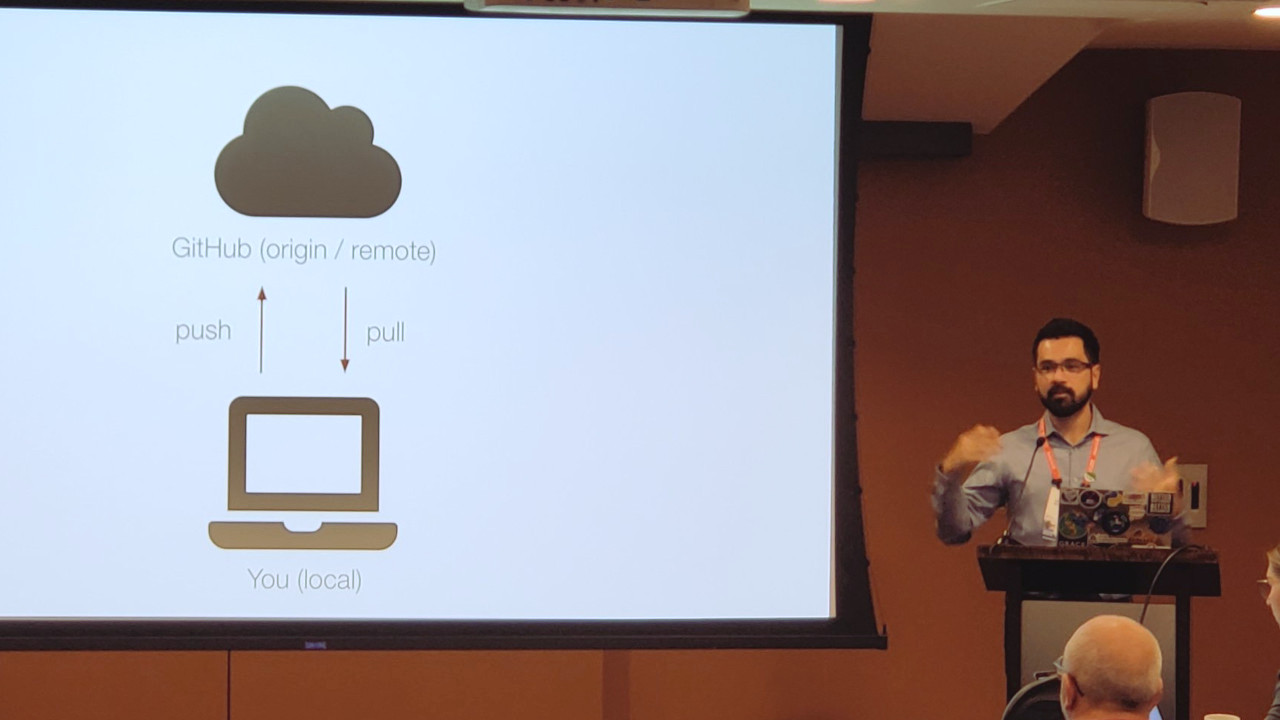
\includegraphics[width=\textwidth]{images/agu-2019-git-lesson.jpg}
  \end{center}
  \caption{
    Foto tirada durante o curso ``Best Practices for Developing and Sustaining
    Your Open-Source Research Software'' que ministrei em 2019 durante o
    \href{https://github.com/agu-ossi/2019-agu-oss}{AGU Fall Meeting} em
    São Francisco, E.U.A.
  }
\end{figure}
\begin{summarybox}[frametitle=\faChalkboardTeacher{}\quad Resumo da experiência de ensino]
  \begin{fa-ul}
    \faChalkboardTeacher & 10 disciplinas de graduação ministradas \\
    \faClock & 17 cursos de curta duração ministrados internacionalmente \\
    \faCheckSquare & Habilitação em pedagogia e técnicas de ensino aplicadas ao
      ensino superior \\
    \faLightbulb & Tópicos ensinados incluem: gravimetria, magnetometria,
    sismologia, sensoriamento remoto, métodos numéricos, programação em Python,
    métodos de campo em geofísica, introdução à geologia, problemas inversos,
    geofísica global e geodinâmica da litosfera.
  \end{fa-ul}
\end{summarybox}

Ensino é a parte que eu mais gosto.
Como eu abordo o ensino.
Citar artigos de pedagogia.
Figura do notebook de ondas sísmicas.
Ensino guiando a pesquisa (imagem do Havaí e trabalho do Gelson).

Crise na geociências.
Fenômeno global citar trabalhos nos EUA e Inglaterra.
Qual é o papel da geofísica além do petróleo.
Ciência de dados.
Aplicações ambientais.
Importância de conceitos de programação para ser cidadão informado no século XXI.

\section{Cursos de curta duração}

\begin{subsummarybox}[frametitle=\faClock{}\quad Cursos e workshops ministrados]
  \begin{paperlist}
    2022 &
      Crafting beautiful maps with PyGMT.
      \textit{EGU 2022}.
      \GitHub{GenericMappingTools/egu22pygmt}
      \\
    ~ &
      A geophysical tour of mid-ocean ridges.
      \textit{Transform 2022} (online).
      \GitHub{leouieda/transform2022}.
      \YouTube{NzJmRlJCNbQ}
      \\
    2021 &
      The Generic Mapping Tools for Geodesy.
      \textit{UNAVCO} (online).
      \GitHub{GenericMappingTools/2021-unavco-course}
      \\
    2020 &
      Let's build a geophysical inversion with Python.
      \textit{IRTG-2379 Graduate School: Modern Inverse Problems},
      \textit{RWTH Aachen University} (online).
      \GitHub{compgeolab/2020-aachen-inverse-problems}
      \\
    ~ &
      The Generic Mapping Tools for Geodesy.
      \textit{UNAVCO} (online).
      \GitHub{GenericMappingTools/2020-unavco-course}.
      \YouTube{EQgxDmCXvj4}
      \\
    ~  &
      From scattered data to gridded products using Verde.
      \textit{Transform 2020} (online).
      \GitHub{fatiando/transform2020}.
      \YouTube{-xZdNdvzm3E}
      \\
    2019 &
      Best Practices for Developing and Sustaining Your Open-Source Research Software.
      \textit{AGU Fall Meeting 2019}.
      \GitHub{agu-ossi/2019-agu-oss}
      \\
    ~  &
      Become a Generic Mapping Tools Contributor Even If You Can't Code.
      \textit{AGU Fall Meeting 2019}
      \\
    ~  &
      The Generic Mapping Tools for Geodesy.
      \textit{Scripps Institution of Oceanography} and \textit{UNAVCO}.
      \GitHub{GenericMappingTools/2019-unavco-course}.
      \YouTube{uPUt4\_kd6m8}
      \\
    ~  &
      Introduction to Python Workshop (Earth Sciences REU program).
      \textit{Department of Geology and Geophysics, \UHM}.
      \GitHub{leouieda/2019-06-reu-python}
      \\
    2018 &
      Best Practices for Modern Open-Source Research Codes.
      \textit{AGU Fall Meeting 2018}.
      \GitHub{agu-ossi/2018-agu-oss}
      \\
    ~  &
      Git and GitHub: What are their uses? Are they worth the effort? Let's find out!
      \textit{ASPRS UHM Student Chapter, \UHM}
      \\
    2017 &
      Introduction to Python.
      \textit{Department of Geology and Geophysics, \UHM}.
      \GitHub{leouieda/python-hawaii-2017}
      \\
    2016 &
      Python for Geologists (SAGEO).
      \textit{Faculdade de Geologia, \UERJ}.
      \GitHub{leouieda/python-geologia-2016}
      \\
    ~  &
      Python como uma ferramenta numérica em Ciências da Terra: uma nova
      abordagem de programação.
      \textit{XVIII Escola de Verão de Geofísica do IAG-USP}.
      \GitHub{leouieda/verao2016}
      \\
    2014 &
      Tópicos de inversão em geofísica.
      \textit{III Semana de Geofísica da UnB}.
      \GitHub{pinga-lab/inversao-unb-2014}
      \\
    2012 &
      Tópicos de inversão em geofísica.
      \textit{XVI Escola de Verão de Geofísica do IAG-USP}.
      \GitHub{pinga-lab/inversao-iag-2012}
  \end{paperlist}
\end{subsummarybox}

Primeira experiência na USP.
Escolas de verão no Brasil.
Software Carpentry.
AGU.
GMT e GMTSAR.
Transform.

\section{Disciplinas de graduação}

\begin{subsummarybox}[frametitle=\faClock{}\quad Disciplinas ministradas]
  \begin{courselist}
    2023--atual  &
      ENVS219: Earth and Environmental Data Science (\textit{em
      desenvolvimento}).
      \textit{University of Liverpool}.
      \\
    2020--atual  &
      ENVS398: Global Geophysics and Geodynamics.
      \textit{University of Liverpool}.
      \GitHub{leouieda/lithosphere}
      \\
    ~ &
    ENVS258: Environmental Geophysics.
      \textit{University of Liverpool}.
      \GitHub{leouieda/remote-sensing}.
      \GitHub{leouieda/gravity-processing}.
      \\
    ~ &
    ENVS386: Geophysical Data Modelling.
      \textit{University of Liverpool}.
      \GitHub{leouieda/ml-intro}.
      \\
    ~ &
      ENVS101/106: Study Skills and GIS (tutorial).
      \textit{University of Liverpool}.
      \\
    2019--2021 &
      ENVS123: Introduction to Geoscience and Earth History.
      \textit{University of Liverpool}.
      \\
    2019--2020  &
      ENVS363: Geophysics Field School.
      \textit{University of Liverpool}.
      \\
    2015--2016 &
      IME03-1366 Matemática Especial I. \textit{\UERJ}.
      \GitHub{mat-esp/about}
      \\
    2014--2016 &
      FGEL04-12422 Geofísica II. \textit{\UERJ}.
      \GitHub{leouieda/geofisica2}
      \\
    ~ &
      FGEL04-12421 Geofísica I. \textit{\UERJ}.
      \GitHub{leouieda/geofisica1}
      \\
    2015 &
      FGEL01-00805 Geologia Geral I. \textit{\UERJ}.
  \end{courselist}
\end{subsummarybox}

Matérias que eu criei.
Material didático.
Paraninfo da turma.
Disciplinas de campo.

PGCAP.
Disciplinas de campo.
Matérias criadas em Liverpool.
Machine learning.
Environmental Data Science em todos os cursos.
Coordenação do curso.


%==============================================================================
\chapter{Atividades de Extensão}
\label{cap_extensao}

Entrevistas nos podcasts, open days.
Parte que está faltando mais e que eu quero investir mais tempo.
Pandemia significou que muitas dessas atividades não estavam acontecendo antes.
Experimento com o imã e Phyphox.


%==============================================================================
\chapter{Conclusão}
\label{cap_conclusao}

Repete resumo dos principais pontos.
Termina com o que eu pretendo conquistar no futuro.

Incluir resumo de ideias de pesquisa (fazer referência ao projeto),
extensão (cursos de programação, videos sobre geofísica) e ensino (introduzir
computação ao longo do currículo, software carpentry no verão, livros abertos,
mesa redonda do futuro da geofísica).

%==============================================================================
\backmatter
\bibliographystyle{apalike-doi}
\bibliography{references}

\end{document}
